\subsection{Netzwerkanalyse}
Mit einer Netzwerkanalyse kann am schnellsten erkannt werden, was auf einem Honeypot passiert ist. Die Netzwerkanalyse kann grundsätzlich auf zwei Wege genutzt werden. Zum einem kann erkannt werden welche Ports verwendet wurden, zum anderen kann über die Payload der Pakete nach Details geforscht werden. Wenn der übertragenen Datenverkehr nicht verschlüsselt ist, kann ein Packet-Sniffer (z.B. WireShark) den kompletten Verkehr aufzeichnen. Fragen, die sich bei der Netzwerkanalyse stellen, sind:

\begin{itemize}
\item Wie viele Pakete wurden aufgezeichnet
\item Welche IP Adressen waren beteiligt
\item Wer kommunizierte mit wem
\item Welche Ports wurden verwendet
\item Welche zeitlichen Abstände befinden sich zwischen den abgesendeten Paketen
\item Wie groß waren die Pakete
\end{itemize} 

\noindent Da bei einem länger aktiven Honeypot eine sehr große Menge an Daten in Log-Files gespeichert werden können, sollte sich nicht auf jeden einzelne Kommunikationsvorgang, sondern eher auf die \emph{top talker} (diejenigen, die am meisten kommuniziert haben) geachtet werden. Packet-Sniffer bieten meist die Möglichkeit nach bestimmten Ziel- oder Quell Adressen, Ports oder Protokollen zu filtern. Der zeitliche Abstand verdächtiger Pakete kann Auskunft geben, ob ein Angriff automatisch oder manuell stattfand. Häufig sind Angriffe, die innerhalb von kurzen Zeitintervallen stattfinden, automatisiert. 
Außerdem sollte auf die Paketgröße geachtet werden. Kleine Pakete sind meist Handshake- Broadcast- oder Protocol-overhead Pakete, und können (je nach zu analysierenden Angriff) ignoriert werden. 

Nachdem die Pakete nach den gewünschten Kriterien gefiltert wurden, kann versucht werden ein Muster aus den verschiedenen Paketen zu erkennen.\\

\begin{figure}[h]
    \centering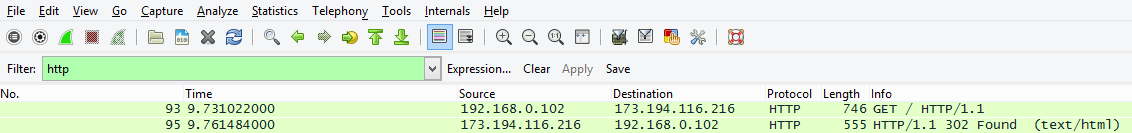
\includegraphics[scale=0.5]{Bilder/Wireshark.png}
  \caption{Packet-Sniffer Wireshark }
  \label{ws}
\end{figure}